This chapter will: describe the existing architecture, namely the technologies involved with the tool such as the VDM AST\footnote{Abstract Syntax Tree} and the intermediate representation of VDM; describe how the existing tool works; describe the five step methodology that was used and repeated in a development cycle; describe the ways in which I have extended the existing tool and detail the implementation of these extensions and finally outline the translation 'recipe'.
\hfill\break
\section{Existing Architecture Description} \label{ead}
\subsection{The VDM AST and Core Modules}
The Abstract Syntax Tree (AST) "is an in-memory representation of the VDM model being worked on"\parencite{OvertureWikiArchitectureDescription} and is made up of a series of classes which implement an AST for VDM. The AST is generally structured like in Fig\ref{fig:AST General Architecture}.
\begin{figure}
        \center{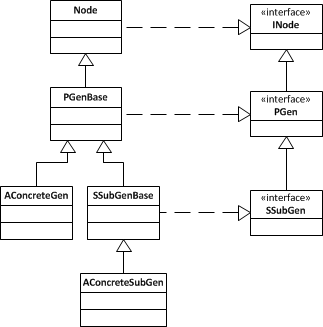
\includegraphics[width=\textwidth]
        {Images/asthierch.png}}
        \caption{\label{fig:AST General Architecture} The AST's General Architecture \parencite{vdmwikiast}}
      \end{figure}.

Nodes have fields which hold information on their values, as well as fields which hold information about, and provide access to, their children and ancestors. Neighbouring nodes - children and ancestor nodes - can be used to infer the structure of the AST surrounding any given node. Child nodes are fields of their parent nodes, this provides the tree structure of the AST. The highest-level class entity in the AST is the abstract \lstinline[language=Java]{Node} class which implements, and provides default definitions for, methods in the \lstinline[language=Java]{INode} interface. This interface defines common behaviour of all nodes in the AST whether they are binary expressions or function patterns. To name but a few, the INode interface contains abstract methods like \lstinline[language=Java]{parent()}, \lstinline[language=Java]{getChildren()} and \lstinline[language=Java]{removeChild()} which all allow for the AST to be manipulated accordingly by visitor classes later. The INode interface also includes abstract \lstinline[language=Java]{apply()} methods to support the visitor pattern for various adaptors, these concepts are explained in detail in section \ref{vp}. The \lstinline[language=Java]{PGen} interface is implemented by \lstinline[language=Java]{PGenBase} which extends \lstinline[language=Java]{Node} and is extended by \lstinline[language=Java]{SSubGenBase} which implements the \lstinline[language=Java]{SSubGen} interface. Evidently then, the structure of the AST is intricate but does provide excellent extensibility for tools such as the one that this project will attempt to implement.

A more concrete example of the AST's structure is the \lstinline[language=Java]{PExp} expressions family of VDM nodes seen in Fig\ref{fig:The AST hierarchy for a binary expression}. This example shows the AST hierarchy for a simple numeric binary expression like $a + b$. The concrete classes \lstinline[language=Java]{APlusNumericBinaryExp} and \lstinline[language=Java]{ATimesNumericBinaryExpIR} are leaf nodes as \lstinline[language=Java]{AConcreteSubGen} was in Fig\ref{fig:AST General Architecture}\begin{figure}
        \center{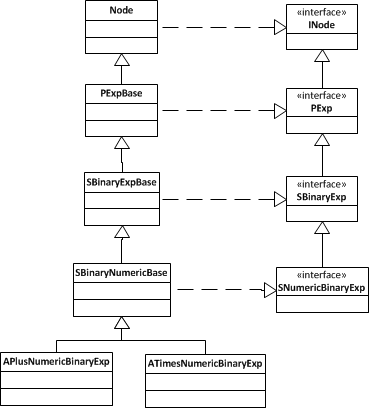
\includegraphics[width=\textwidth]
        {Images/vdmwikibinh.png}}
        \caption{\label{fig:The AST hierarchy for a binary expression} The AST hierarchy for a binary expression, in this case plus and times. \parencite{vdmwikiast}}
      \end{figure}

VDM is made up of a number of core modules, seen in Fig\ref{fig:VDM Modules Architecture}, which all work to build and manipulate the AST. It is worth mentioning that these modules are implemented in Overture, the Eclipse based IDE and VDM-SL platform. This project branches from the Overture GitHub, namely the cth/isagen branch maintained by Casper Thule Hansen,\parencite{VDM2ISAGit} and the entire development is an extension of the Overture package's \ttfamily\hl{CodeGen} module.\rmfamily\begin{figure}
        \center{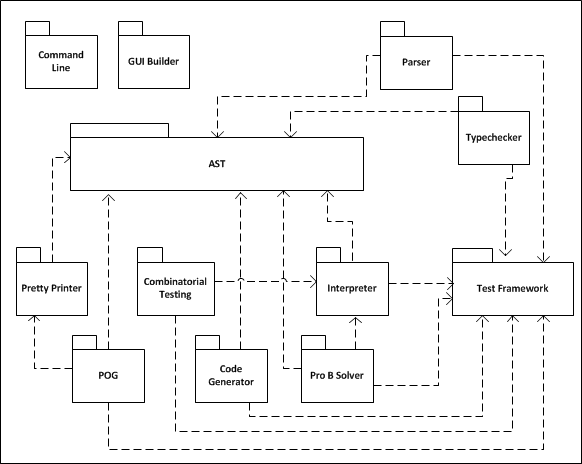
\includegraphics[width=\textwidth]
        {Images/vdmmodules.png}}
        \caption{\label{fig:VDM Modules Architecture} The Architecture of Core VDM Modules \parencite{OvertureWikiArchitectureDescription}}
      \end{figure}.
Fundamentally, all modules are built around the Abstract Syntax Tree (AST), all modules are written in pure Java. A very brief overview of the most important modules is as follows: \begin{itemize}
	\item The \ttfamily\hl{Parser} \rmfamily reads a VDM model and constructs its AST.
	\item After the operation of the \ttfamily\hl{Parser} \rmfamily, an AST is built. The \ttfamily\hl{Typechecker} \rmfamily module validates this AST and assigns types to each node, one such check might test if a given union type contains a Boolean type. An output of this stage is an Intermediate Representation, see \ref{cgair}.
	\item The \ttfamily\hl{Interpreter} \rmfamily module is responsible for executing the AST constructed from VDM Models by the \ttfamily\hl{Parser} \rmfamily, and interacting with the user.
	\end{itemize}


The main module of interest to this project in particular however; is the \ttfamily\hl{Code Generator} \rmfamily, in which lies the base \ttfamily\hl{Code Generator} \rmfamily that generates an Intermediate Representation (IR), and the \lstinline[language=Java]{IsaGen} package which manipulates that IR and contains all of the code written for the entirety of this project.

\subsection{Code Generator \& Intermediate Representation} \label{cgair}
After the \ttfamily\hl{Parser} \rmfamily, \ttfamily\hl{Typechecker} \rmfamily and their subsequent modules have completed operation \footnote{But before any output is produced by the \ttfamily\hl{Interpreter} \rmfamily or its subsequent modules.}, an Intermediate Representation (IR) is output. An IR is commonly used in programming languages to provide extensibility for Code Generators such as the Isabelle/HOL generator in question. An IR is a representation of a program between the source and target programming languages; after VDM has been compiled into an AST but before it is translated into Java or C++, or HOL here. The IR is independent of its source or target languages and is meant to provide a common ground, an interface of sorts between different tools and languages operating on one AST, similar is the way that Latin is used in the classification of wildlife, \lstinline[language=Java]{AAndBoolBinaryExpIR} IR node is an \lstinline[language=Java]{AAndBoolBinaryExpIR} node in both VDM and Isabelle ASTs. The IR allows the translation tool to analyse and manipulate an AST without repeatedly translating to and from VDM and Isabelle and allows the tool to have a pre-type-checked AST to work with. This is beneficial as we do not need to type check again in Isabelle after translation, the translation is broken up into manageable parts. A type-checked binary expression in IR is still a validated and type checked binary expression in Isabelle, or else it would not have been parsed to the IR AST by the \ttfamily\hl{Parser} \rmfamily and \ttfamily\hl{Typechecker} \rmfamily.

The \ttfamily\hl{Code Generator} \rmfamily module contains a base \ttfamily\hl{Code Generator} \rmfamily class which is responsible for providing access to the IR. Sub classing this class gives access to the IR and some valuable AST settings information. This Isabelle/HOL translator, which works within the \ttfamily\hl{Code Generator} \rmfamily module, approximately follows a five-step methodology originally proposed in the 13th Overture Workshop\parencite{overtureproceedings} and reads like so: [1] set-up, [2] add new nodes, [3] transform the IR, [4] generate syntax, [5] validate the translation.  

\begin{figure}
        \center{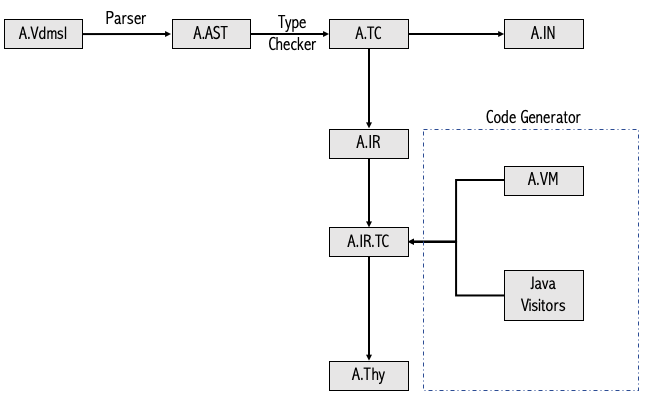
\includegraphics[width=\textwidth]
        {Images/FileOuts.png}}
        \caption{\label{fig:OES} The output progression of the A.vdmsl file.}
\end{figure}

\section{Methodology}
This section will describe the established methodology closely followed by this project as well as explanations of tools and technologies involved in its implementation.

	\subsection{	[1] Set-up a CGP extension} \label{s1}
	Have a class which extends the \lstinline[language=Java]{CodeGenBase} class and create a new template manager which will provide access to the template structure class provided by the \ttfamily\hl{Code Generator} \rmfamily module. Lastly, set up a basic testing facility, Overture, the Eclipse based IDE and VDM-SL interpreter utility in which we write VDM-SL, provides a test framework, this should be used to set up the tests. 
	\subsection{	[2] Add New Nodes}
	If the target language is significantly different from the first, then new nodes may need to be created and added to the AST. In the case of Isabelle, new nodes were needed quite often. In fact, almost every operation required addition of new Expression, Definition or Pattern nodes to the IR AST. This is because, as mentioned previously, an Isabelle translation requires explicit translation of every construct, for example invariants, pre and post conditions are translated as separate functions - contrary to how VDM handles say, functions, with pre and post conditions attached to the definition as VDM AST node fields.
	\subsection{	[3] Transform the IR} \label{ttir}
	This step transforms the AST so that the target language can be generated from it in the next stage. Constructs that are not supported in the target language are transformed away and fields and nodes are adjusted, or constructs removed altogether. There are two types of transformation applied to the AST: 
   	\begin{itemize}
	   \item A partial transformation. A partial transformation is trivial to apply but is limited in the way that it can only change the internal structure of the node - like fields, method overrides and so on. A partial transformation does not make large changes to the AST and so does not interfere greatly with its structure. Rarely, only minor adjustments need be made to an ancestor or a child of a partially transformed construct and this is often easily or even automatically achieved with implemented get and set methods.
	   \item A total transformation. Total transformations can change the node itself; the node can be transformed into a different node through type casts for example, removed and replaced with a different node or removed from the tree entirely. Total transformations are difficult to perform and, as I discovered during my implementation of the tool, volatile and vulnerable to anomalous behaviour, sub nodes of the node must on occasion be subsequently changed significantly according to the changes made to their ancestor. The following code snippet from the overture git shows how to apply transformations.
	   \begin{lstlisting}
	   	List<ExtIrClassDeclStatus> transformed = new Vector<>();

		for (IRClassDeclStatus status : untransformed)
		{
		  // Partial transformation applied directly
		  PartialTransformationFoo t1 = new PartialTransformationFoo();
		  generator.applyPartialTransformation(status, t1);

		  // Total transformations need wrapping
		  ExtIrClassDeclStatus eStatus = new ExtIrClassDeclStatus(status);
		  TotalTransformationBar t2 = new TotalTransformationBar();
		  generator.applyTotalTransformation(eStatus, t2);
		  transformed.add(eStatus);
		}
	  	\end{lstlisting}\parencite{vdmwikicgp}
 	\end{itemize}
	Total transformations need extra work within the \lstinline[language=Java]{TotalTransformationBar} to harmonize the tree with the change to its nodes. Transformations themselves take the form of visitor classes, the \lstinline[language=Java]{PartialTransformationFoo} class above is a visitor class. The visitor pattern is important and so it is given its own section in \ref{vp}.

	\subsubsection{The Visitor Pattern} \label{vp}
	Manipulating the VDM AST directly is highly discouraged, the system of modules and their dependencies is far too complex to handle direct changes to its central component. The idea of a visitor design pattern is to detach an algorithm from the data that it operates on, in this case to detach the VDM AST from code generation transformations performing potentially erroneous meddling. As mentioned in section \ref{ead}, the \lstinline[language=Java]{INode} interface that is the highest level of abstraction in the VDM AST enforces \lstinline[language=Java]{apply()} methods. All Nodes in the AST have \lstinline[language=Java]{apply()} methods as they enable the visitor pattern. Where before, something like \lstinline[language=Java]{node.changeParent()}, becomes instead \lstinline[language=Java]{node.apply(parentChangeVisitor)} where \lstinline[language=Java]{parentChangeVisitor} is a Java class with methods that change the parent of a node. Almost every time that we interact with the AST this pattern is used. The \lstinline[language=Java]{apply()} method, implemented by each node, allows each node of the AST to control the way in which it is individually transformed according to its own subtle intricacies that would not be, nor should have to be, strictly adhered to by external classes. The \lstinline[language=Java]{apply()} method, and by extension the visitor pattern, hence gives control of any interaction with the AST, over to the AST nodes' classes, each of which know precisely how to handle interaction safely in their own unique way, because of this, the AST is never damaged or malformed. 

	The AST classes will only accept a class in their \lstinline[language=Java]{apply()} functions if that class is a visitor. A class is identified as a visitor by extending, sub-classing, an adaptor class in the \lstinline[language=Java]{org.overture.ast.analysis} package, an adaptor class \textbf{adapts} AST interaction by visitors into a safe one. More on the various analysis adaptor classes in this package is discussed later in this section. In order for a visitor to be able to interact with different types and families of nodes, they must be equipped with a method containing functionality for the \emph{case} that certain nodes might be encountered.

	Cases are a powerful construct within the visitor pattern, they allow the programmer to do away with exceedingly long control blocks used to test for the presence of specific nodes, any large code blocks can be stored in a separate visitor class containing case methods for what to do for each different node family or type. Each class in the \lstinline[language=Java]{org.overture.ast.analysis} package is filled with case methods for every type of node. The \lstinline[language=Java]{DepthFirstAnalysisAdaptor} class contains approximately $16,000$ lines of code the majority of which are empty or basic case methods which are overridable so that the sub-classed visitor can add its own functionality for that node case. Each method takes as a parameter, a node of the type that it is the case for. To name but a minute few in this class:
	\begin{lstlisting}[language=Java]
	caseARealPatternIR(ARealPatternIR)
	caseARecordDeclIR(ARecordDeclIR)
	caseARecordModExpIR(ARecordModExpIR)
	caseARecordModifierIR(ARecordModifierIR)
	caseARecordPatternIR(ARecordPatternIR)
	caseARecordTypeIR(ARecordTypeIR)
	caseARemNumericBinaryExpIR(ARemNumericBinaryExpIR)
	caseARenamedDeclIR(ARenamedDeclIR)
	caseARepeatTraceDeclIR(ARepeatTraceDeclIR)
	caseAReturnStmIR(AReturnStmIR)
	caseAReverseUnaryExpIR(AReverseUnaryExpIR)
	caseASameBaseClassExpIR(ASameBaseClassExpIR)
	caseASameClassExpIR(ASameClassExpIR)
	\end{lstlisting}
	If, for example, the programmer would like to create a visitor that counts the number of fields in \lstinline[language=Java]{ARecordDeclIR}\footnote{The IR node for a declaration of a record type.} then they would write a class like so:
	\begin{lstlisting}[language=Java]
	public class EmptySeqVisitor extends AnalysisAdaptor {

	  int nodeCount;
	  
	  @Override
	  public void caseARecordDeclIR(ARecordDeclIR node)
	      throws AnalysisException {
	  
	    nodeCount = node.getFields().size();
	    //_fields is a NodeList<AFieldDeclIR>() field in ARecordDeclIR. NodeList is a VDM class in the AST package implementing list functionality.
	    
	  }
	  
	}
	\end{lstlisting}

	The \lstinline[language=Java]{org.overture.ast.analysis} package contains additional classes, adaptors, to \lstinline[language=Java]{AnalysisAdaptor} which can be extended to provide various AST interactions, parameter passing, return values, or both. 
	\begin{enumerate}
		\item \lstinline[language=Java]{AnalysisAdaptor} The easiest way to create a visitor to the AST, it takes no parameters and the return type of its overridden methods are always void. Such a visitor can be used, for example, to count occurrences of a type of node by incrementing a field as the visitor encounters a node of a certain type. 
		\item \lstinline[language=Java]{QuestionAdaptor<Q>} Allows the visitor to pass information to the AnalysisAdaptor as a generic type parameter, though this parameter must be the same for all cases in a given visitor. In a question visitor the parameter object \lstinline[language=Java]{<Q>} is passed as a second parameter to every method in the visitor. It can be used to check the equality of a node or its fields, to set a parameter of a node to a different value and so on.
		\item \lstinline[language=Java]{AnswerAdaptor<A>} Allows the visitor to define a return type and gather data from the AST so long as the data is of type \lstinline[language=Java]{<A>}. Every method in the visitor has a return type of \lstinline[language=Java]{<A>}. Extending this class requires the visitor to implement two additional methods \lstinline[language=Java]{createNewReturnValue(INode node)} and \lstinline[language=Java]{createNewReturnValue(Object node)}, as something must be returned, these methods are invoked when no other case is matched.
		\item \lstinline[language=Java]{QuestionAnswerAdaptor<Q,A>} As may be evident from the name, a visitor that is a subclass of this class can both pass parameters of type \lstinline[language=Java]{<Q>} and take a return type of \lstinline[language=Java]{<A>}. This class allows for the most flexibility of the three and must implement the same methods as the proceeding classes in this list.
		\item \lstinline[language=Java]{DepthFirstAnalysisAdaptor} This is used frequently in this project; this adaptor allows a visitor to perform a depth first tree traversal of the AST and perform analysis as it does so. A visitor that is a subclass of this class is given the same methods to implement and override as the \lstinline[language=Java]{AnalysisAdaptor} class with the addition of \lstinline[language=Java]{public void setVisitedNodes(Set<INode> value)} and the field \lstinline[language=Java]{_visitedNodes} which allow sub-classed visitors to access the nodes visited during the depth first tree traversal. This is a particularly useful class for modifying the AST, nodes that need to be worked on can be on wildly different sub-trees due to the differences between Isabelle and VDM.
		\item \lstinline[language=Java]{DepthFirstAnalysisAdaptorAnswer<A>} Performs a depth first analysis of the tree with the addition of answer functionality described in  \lstinline[language=Java]{AnswerAdaptor<A>} above.
		\item \lstinline[language=Java]{DepthFirstAnalysisAdaptorQuestion<Q>} Performs a depth first analysis of the tree with the addition of question functionality described in  \lstinline[language=Java]{QuestionAdaptor<A>} above.
		\item \lstinline[language=Java]{DepthFirstAnalysisAdaptorQuestionAnswer<Q,A>} Performs a depth first analysis of the tree with the addition of question/answer functionality described in  \lstinline[language=Java]{QuestionAnswerAdaptor<A>} above.
	\end{enumerate} 


	\subsection{	[4] Generate Target Language Syntax}
	Now that the AST has been transformed into a state ready to be translated into an AST of its target language, it is passed into the syntax generation framework of the \ttfamily\hl{Code Generator} \rmfamily module. At this stage the \ttfamily\hl{Code Generator} \rmfamily module traverses the IR AST and creates translated target language code as a String for each node. The \ttfamily\hl{Code Generator} \rmfamily detects the node's type and then creates code for it by populating pre-defined Apache Velocity templates, see \ref{av} for a description of Apache Velocity and its application to this project.
	\subsubsection{Apache Velocity} \label{av}
	Apache Velocity is a Java based template engine in which a \ttfamily\hl{.vm} \rmfamily file is written containing Velocity syntax, the velocity syntax accesses variables defined in Java code and allows the programmer to interweave their values with appropriate syntax, lexicon and document structure to create the desired output string or file. Some example Velocity syntax is:
	\hfill\break
	\begin{lstlisting}[language=Velocity]
		($Isa.trans($node.Left) \<and> $Isa.trans($node.Right))
	\end{lstlisting} 
	\hfill\break
	This creates essentially place holders for the result of Java computations that will create a value for a Java translation method \lstinline[language=Java]{trans(INode node)} which will have passed into it the node which is the left hand side value of the binary \ttfamily\hl{and} \rmfamily expression followed by the Isabelle/HOL symbol for \ttfamily\hl{and} \rmfamily \lstinline[language=Isabelle, mathescape]{\<and>}\footnote{which will be translated into the HOL symbol $\wedge$} followed by the node which is the right hand side of the \ttfamily\hl{and} \rmfamily expression - we will get something like $A \wedge B$ in Isabelle. The and template is a trivial example but templates as complex as entire function definition structures can be achieved.  
	\hfill\break
	\hfill\break
	\hfill\break
	\hfill\break
	\textbf{Velocity}
	\begin{lstlisting}[language=Velocity, caption=The Velocity template for function declarations. Below is a translation showing how one such template is used in practice.]
	#macro ( transIdentifiers $node )
	#foreach($p in $node.FormalParams)
	$Isa.trans($p.pattern)##
	#end
	#end

	definition
	#if ("$Isa.transTypeParams($node.MethodType.Params)" == "")
		$node.Name :: "$Isa.trans($node.MethodType.Result)"
	#else
		$node.Name :: "$Isa.transTypeParams($node.MethodType.Params) \<Rightarrow> $Isa.trans($node.MethodType.Result)"
	#end
	    where
	    "$node.Name #transIdentifiers($node) \<equiv> $Isa.trans($node.Body)"
	\end{lstlisting} 

	\textbf{Translation}
	\hfill\break
	\hfill\break
	\pagecolor{bgcolor}
	\ttfamily
	\syntaxNULL{}\gutter{\ \ \ \ 1{|}\ }\syntaxKEYWORDA{theory}{\ }A\hspace*{\fill}\\
	\gutter{\ \ \ \ 2{|}\ }{\ }{\ }{\ }{\ }{\ }{\ }\syntaxKEYWORDB{imports}{\ }VDMToolkit\hspace*{\fill}\\
	\gutter{\ \ \ \ 3{|}\ }{\ }{\ }{\ }{\ }\syntaxKEYWORDB{begin}\hspace*{\fill}\\
	\gutter{\ \ \ \ 4{|}\ }\hspace*{\fill}\\
	\gutterH{\ \ \ \ 5{|}\ }\hspace*{\fill}\\
	\gutter{\ \ \ \ 6{|}\ }{\ }{\ }{\ }{\ }\syntaxKEYWORDA{definition}\hspace*{\fill}\\
	\gutter{\ \ \ \ 7{|}\ }{\ }{\ }{\ }{\ }{\ }{\ }f{\ }\syntaxOPERATOR{::}{\ }\syntaxLITERALA{"VDMNat}\hspace*{\fill}\\
	\gutter{\ \ \ \ 8{|}\ }\syntaxLITERALA{{\ }{\ }}\syntaxLITERALA{{\ }{\ }}\syntaxLITERALA{{\ }}\syntaxLITERALA{\usebox{\backslashbox}}\syntaxLITERALA{\usebox{\lessthan}}\syntaxLITERALA{R}\syntaxLITERALA{i}\syntaxLITERALA{g}\syntaxLITERALA{h}\syntaxLITERALA{t}\syntaxLITERALA{a}\syntaxLITERALA{r}\syntaxLITERALA{r}\syntaxLITERALA{o}\syntaxLITERALA{w}\syntaxLITERALA{\usebox{\greaterthan}}\syntaxLITERALA{{\ }}\syntaxLITERALA{V}\syntaxLITERALA{D}\syntaxLITERALA{M}\syntaxLITERALA{N}\syntaxLITERALA{a}\syntaxLITERALA{t}\hspace*{\fill}\\
	\gutter{\ \ \ \ 9{|}\ }\syntaxLITERALA{{\ }{\ }}\syntaxLITERALA{{\ }{\ }}\syntaxLITERALA{{\ }}\syntaxLITERALA{\usebox{\backslashbox}}\syntaxLITERALA{\usebox{\lessthan}}\syntaxLITERALA{R}\syntaxLITERALA{i}\syntaxLITERALA{g}\syntaxLITERALA{h}\syntaxLITERALA{t}\syntaxLITERALA{a}\syntaxLITERALA{r}\syntaxLITERALA{r}\syntaxLITERALA{o}\syntaxLITERALA{w}\syntaxLITERALA{\usebox{\greaterthan}}\syntaxLITERALA{{\ }}\syntaxLITERALA{V}\syntaxLITERALA{D}\syntaxLITERALA{M}\syntaxLITERALA{N}\syntaxLITERALA{a}\syntaxLITERALA{t}\hspace*{\fill}\\
	\gutterH{\ \ \ 10{|}\ }\syntaxLITERALA{{\ }{\ }}\syntaxLITERALA{{\ }{\ }}\syntaxLITERALA{"}\hspace*{\fill}\\
	\gutter{\ \ \ 11{|}\ }{\ }{\ }{\ }{\ }{\ }{\ }{\ }{\ }\syntaxKEYWORDB{where}\hspace*{\fill}\\
	\gutter{\ \ \ 12{|}\ }{\ }{\ }{\ }{\ }{\ }{\ }{\ }{\ }\syntaxLITERALA{"f{\ }x{\ }y{\ }{\ }\usebox{\backslashbox}\usebox{\lessthan}equiv\usebox{\greaterthan}{\ }x"}\hspace*{\fill}\\
	\gutter{\ \ \ 13{|}\ }\hspace*{\fill}\\
	\gutter{\ \ \ 14{|}\ }\hspace*{\fill}\\
	\gutterH{\ \ \ 15{|}\ }{\ }{\ }{\ }{\ }\syntaxKEYWORDA{definition}\hspace*{\fill}\\
	\gutter{\ \ \ 16{|}\ }{\ }{\ }{\ }{\ }{\ }{\ }pre\usebox{\underscorebox}f{\ }\syntaxOPERATOR{::}{\ }\syntaxLITERALA{"VDMNat}\hspace*{\fill}\\
	\gutter{\ \ \ 17{|}\ }\syntaxLITERALA{{\ }{\ }}\syntaxLITERALA{{\ }{\ }}\syntaxLITERALA{{\ }}\syntaxLITERALA{\usebox{\backslashbox}}\syntaxLITERALA{\usebox{\lessthan}}\syntaxLITERALA{R}\syntaxLITERALA{i}\syntaxLITERALA{g}\syntaxLITERALA{h}\syntaxLITERALA{t}\syntaxLITERALA{a}\syntaxLITERALA{r}\syntaxLITERALA{r}\syntaxLITERALA{o}\syntaxLITERALA{w}\syntaxLITERALA{\usebox{\greaterthan}}\syntaxLITERALA{{\ }}\syntaxLITERALA{V}\syntaxLITERALA{D}\syntaxLITERALA{M}\syntaxLITERALA{N}\syntaxLITERALA{a}\syntaxLITERALA{t}\hspace*{\fill}\\
	\gutter{\ \ \ 18{|}\ }\syntaxLITERALA{{\ }{\ }}\syntaxLITERALA{{\ }{\ }}\syntaxLITERALA{{\ }}\syntaxLITERALA{\usebox{\backslashbox}}\syntaxLITERALA{\usebox{\lessthan}}\syntaxLITERALA{R}\syntaxLITERALA{i}\syntaxLITERALA{g}\syntaxLITERALA{h}\syntaxLITERALA{t}\syntaxLITERALA{a}\syntaxLITERALA{r}\syntaxLITERALA{r}\syntaxLITERALA{o}\syntaxLITERALA{w}\syntaxLITERALA{\usebox{\greaterthan}}\syntaxLITERALA{{\ }}\syntaxLITERALA{\usebox{\backslashbox}}\syntaxLITERALA{\usebox{\lessthan}}\syntaxLITERALA{b}\syntaxLITERALA{o}\syntaxLITERALA{o}\syntaxLITERALA{l}\syntaxLITERALA{\usebox{\greaterthan}}\syntaxLITERALA{"}\hspace*{\fill}\\
	\gutter{\ \ \ 19{|}\ }{\ }{\ }{\ }{\ }{\ }{\ }{\ }{\ }\syntaxKEYWORDB{where}\hspace*{\fill}\\
	\gutterH{\ \ \ 20{|}\ }{\ }{\ }{\ }{\ }{\ }{\ }{\ }{\ }\syntaxLITERALA{"pre\usebox{\underscorebox}f{\ }x{\ }y{\ }{\ }\usebox{\backslashbox}\usebox{\lessthan}equiv\usebox{\greaterthan}{\ }(isa\usebox{\underscorebox}invVDMNat{\ }x{\ }\usebox{\backslashbox}\usebox{\lessthan}and\usebox{\greaterthan}{\ }isa\usebox{\underscorebox}invVDMNat{\ }y)"}\hspace*{\fill}\\
	\gutter{\ \ \ 21{|}\ }\hspace*{\fill}\\
	\gutter{\ \ \ 22{|}\ }\hspace*{\fill}\\
	\gutter{\ \ \ 23{|}\ }{\ }{\ }{\ }{\ }\syntaxKEYWORDA{definition}\hspace*{\fill}\\
	\gutter{\ \ \ 24{|}\ }{\ }{\ }{\ }{\ }{\ }{\ }post\usebox{\underscorebox}f{\ }\syntaxOPERATOR{::}{\ }\syntaxLITERALA{"VDMNat}\hspace*{\fill}\\
	\gutterH{\ \ \ 25{|}\ }\syntaxLITERALA{{\ }{\ }}\syntaxLITERALA{{\ }{\ }}\syntaxLITERALA{{\ }}\syntaxLITERALA{\usebox{\backslashbox}}\syntaxLITERALA{\usebox{\lessthan}}\syntaxLITERALA{R}\syntaxLITERALA{i}\syntaxLITERALA{g}\syntaxLITERALA{h}\syntaxLITERALA{t}\syntaxLITERALA{a}\syntaxLITERALA{r}\syntaxLITERALA{r}\syntaxLITERALA{o}\syntaxLITERALA{w}\syntaxLITERALA{\usebox{\greaterthan}}\syntaxLITERALA{{\ }}\syntaxLITERALA{V}\syntaxLITERALA{D}\syntaxLITERALA{M}\syntaxLITERALA{N}\syntaxLITERALA{a}\syntaxLITERALA{t}\hspace*{\fill}\\
	\gutter{\ \ \ 26{|}\ }\syntaxLITERALA{{\ }{\ }}\syntaxLITERALA{{\ }{\ }}\syntaxLITERALA{{\ }}\syntaxLITERALA{\usebox{\backslashbox}}\syntaxLITERALA{\usebox{\lessthan}}\syntaxLITERALA{R}\syntaxLITERALA{i}\syntaxLITERALA{g}\syntaxLITERALA{h}\syntaxLITERALA{t}\syntaxLITERALA{a}\syntaxLITERALA{r}\syntaxLITERALA{r}\syntaxLITERALA{o}\syntaxLITERALA{w}\syntaxLITERALA{\usebox{\greaterthan}}\syntaxLITERALA{{\ }}\syntaxLITERALA{V}\syntaxLITERALA{D}\syntaxLITERALA{M}\syntaxLITERALA{N}\syntaxLITERALA{a}\syntaxLITERALA{t}\hspace*{\fill}\\
	\gutter{\ \ \ 27{|}\ }\syntaxLITERALA{{\ }{\ }}\syntaxLITERALA{{\ }{\ }}\syntaxLITERALA{{\ }}\syntaxLITERALA{\usebox{\backslashbox}}\syntaxLITERALA{\usebox{\lessthan}}\syntaxLITERALA{R}\syntaxLITERALA{i}\syntaxLITERALA{g}\syntaxLITERALA{h}\syntaxLITERALA{t}\syntaxLITERALA{a}\syntaxLITERALA{r}\syntaxLITERALA{r}\syntaxLITERALA{o}\syntaxLITERALA{w}\syntaxLITERALA{\usebox{\greaterthan}}\syntaxLITERALA{{\ }}\syntaxLITERALA{\usebox{\backslashbox}}\syntaxLITERALA{\usebox{\lessthan}}\syntaxLITERALA{b}\syntaxLITERALA{o}\syntaxLITERALA{o}\syntaxLITERALA{l}\syntaxLITERALA{\usebox{\greaterthan}}\syntaxLITERALA{"}\hspace*{\fill}\\
	\gutter{\ \ \ 28{|}\ }{\ }{\ }{\ }{\ }{\ }{\ }{\ }{\ }\syntaxKEYWORDB{where}\hspace*{\fill}\\
	\gutter{\ \ \ 29{|}\ }{\ }{\ }{\ }{\ }{\ }{\ }{\ }{\ }\syntaxLITERALA{"post\usebox{\underscorebox}f{\ }x{\ }y{\ }RESULT{\ }{\ }\usebox{\backslashbox}\usebox{\lessthan}equiv\usebox{\greaterthan}{\ }(isa\usebox{\underscorebox}invVDMNat{\ }x{\ }\usebox{\backslashbox}\usebox{\lessthan}and\usebox{\greaterthan}{\ }\hspace*{\fill}(isa\usebox{\underscorebox}invVDMNat{\ }\hspace*{\fill}y{\ }\usebox{\backslashbox}\usebox{\lessthan}and\usebox{\greaterthan}{\ }isa\usebox{\underscorebox}invVDMNat{\ }RESULT))"}\hspace*{\fill}\\
	\gutterH{\ \ \ 30{|}\ }\hspace*{\fill}\\
	\gutter{\ \ \ 31{|}\ }{\ }{\ }{\ }{\ }\syntaxKEYWORDB{end}\hspace*{\fill}\\
	\mbox{}
	\hfill\break
	\rmfamily
	By this mechanism, the \ttfamily\ttfamily\hl{Code Generator} \rmfamily \rmfamily module traverses the AST and populates the templates while the subsequent steps transform the nodes in the AST by computing and manipulating them in order to provide Velocity with the correct variable values. The purpose of the subsequent steps are to prevent the programmer from having to write large velocity files, a well organised visitor pattern and translator should make their target velocity templates as short as possible, one praise of this project is that the velocity files never exceed any more than $19$ lines of code and are approximately $2.67$, rounded to $3$, lines long on average, this includes white-space. Fig\ref{fig:toolStructure} shows an in detail diagram of these steps' outputs.

	\subsection{	[5] Validate} \label{vdt}
	The validation step involves comparison of the output with a known correct result file. Result files are kept very simple and each construct is separate, for example we have one file to test \lstinline[language=Java]{AIntNumericBasicTypeIR} node translation and it is kept as simple as possible. All test files have the \lstinline[language=Java]{.vdmsl} file extension and have one corresponding \lstinline[language=Java]{.vdmsl.result} file which contains the expected translation of a construct. For example, the file \lstinline[language=Java]{Int.vdmsl} has a corresponding result file \lstinline[language=Java]{Int.vdmsl.result}. 
	\begin{vdmsl}[label=lst:Int.vdmsl,caption=Int.vdmsl]
	types
	XType = int;
	\end{vdmsl}
	\begin{vdmsl}[label=lst:Int.vdmsl.result, caption=Int.vdmsl.result]
	{"translation":"theory DEFAULT
	imports VDMToolkit
	begin

	type_synonym XType \= \"VDMInt\"




	definition
	    inv_XType :: \"(XType) \\<Rightarrow> \\<bool> \"
	    where
	    \"inv_XType x \\<equiv> isa_invTrue x\"

	end","errors":false}
	\end{vdmsl}  
	A test passes if the output of the first file, after running through all of the core modules and the translation tool, matches the second.

	\section{Previous Tool Implementation Work}
	\subsection{Previously Completed Step [1] Set-up A CGP Extension}

	Before starting this project, Casper Thule Hansen, PhD Researcher of Aarhus University Denmark\parencite{casper}, had completed the important and tricky first step of the methodology described in \ref{s1}.\parencite{VDM2ISAGit}
	\begin{figure}
        \center{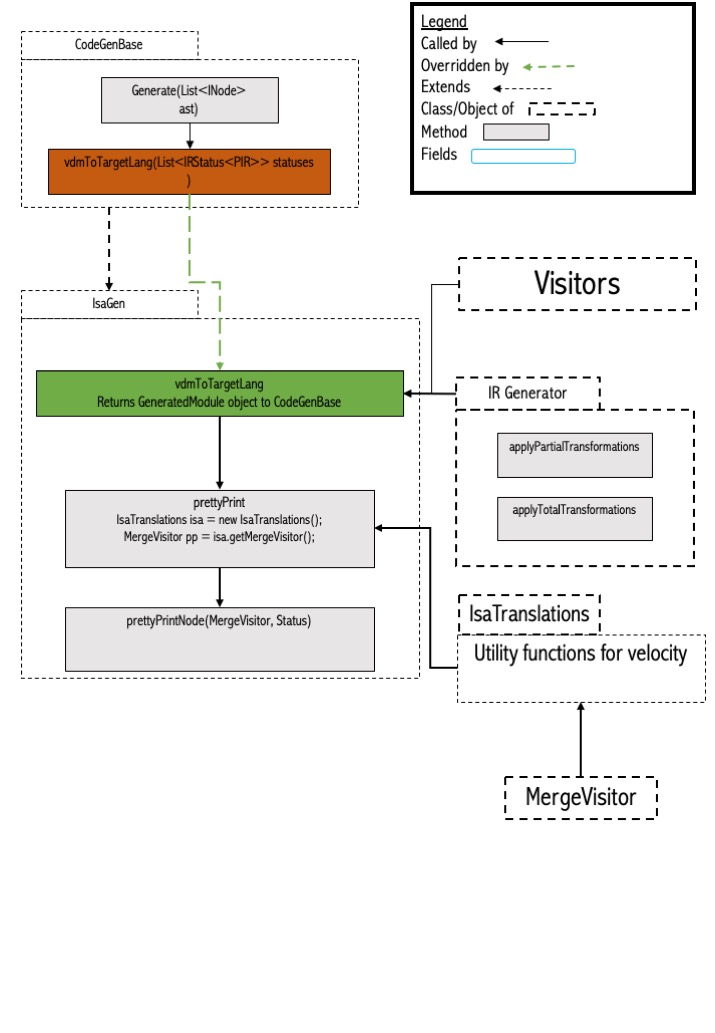
\includegraphics[width=\textwidth]
        {Images/toolStructure.jpg}}
        \caption{\label{fig:toolStructure} The tools structure at the set up stage. \parencite{vdmwikiast}}
     \end{figure}.
    As mentioned in \ref{s1} this is the first step in creating a CGP (Code Generation Platform) extension.\ref{fig:toolStructure} \lstinline[language=Java]{IsaGen}, extends the \lstinline[language=Java]{CodeGenBase} class and the \lstinline[language=Java]{IsaTranslations} class serves as a template manager, this class provides access to the template structure provided by the \ttfamily\hl{Code Generator} \rmfamily module by creating a \lstinline[language=Java]{MergeVisitor} object as a field as well as a list of callable templates, \lstinline[language=Java]{TemplateCallable[] templateCallables} from the \lstinline[language=Java]{org.overture.codegen.merging.TemplateCallable} package in the CGP module, for accessing the various Velocity templates for each node.

    The \lstinline[language=Java]{IsaGen} class overrides the \lstinline[language=Java]{genVDMToTargetLang} method\footnote{See appendix \ref{beforecode}, section \ref{IsaGenbefore}to see \lstinline[language=Java]{genVdmToTargetLang} before development, and appendix \ref{aftercode}, section \ref{IsaGenafter}, for after development} in \lstinline[language=Java]{CodeGenBase}. This method is used by \lstinline[language=Java]{CodeGenBase} and the CGP to generate the target language data. By overriding it, it becomes our main point of interaction with the CGP and so this is where we perform our transformations. We do so by placing visitor classes in this method, taking \lstinline[language=Java]{status} as an argument. 

    Once this method has initialised the fields of a \lstinline[language=Java]{GeneratedModule} object, it is returned to the calling method in \lstinline[language=Java]{CodeGenBase}, \lstinline[language=Java]{generate()}, which is used by \lstinline[language=Java]{CodeGenBase} in a series of steps by the CGP to create the target language output.
   
	The \lstinline[language=Java]{getInfo()} method provides access to AST settings while the parameter \lstinline[language=Java]{List<IRStatus<PIR>> statuses} provides access to the AST itself. The method generates the IR using the CGP and Typechecker module through several calls to CGP methods during the lambda function at the top of the method. 

	As the final step in stage one, a test framework had also been set up. The test that I used was the JUnit class \lstinline[language=Java]{IsaGenParamTest}. The test strategy was that all tests should pass and before this project one already did, integer, as described later in this section\footnote{The full class can be seen in appendix \ref{testing}}. It is necessary to understand that this test class was set up as an array of skipped tests, the strategy was to activate a test, make it pass and then continue to the next.\footnote{See appendix \ref{testing} for the full code.}

	
	\subsection{Previous Work on Step [2] Add New Nodes \& Step [3] Transform The IR} \label{pwos}

	Some parts of the transformation step described in \ref{ttir}, were also implemented prior to this project.	As the tool goes over the AST it applies visitor classes to its nodes. Total transformations are applied to each status, by the  \lstinline[language=Java]{GroupMutRecs} visitor, recursion cycles in the AST's structure are transformed away before translation to Isabelle. The \lstinline[language=Java]{SortDependencies} visitor is applied to \lstinline[language=Java]{AModuleDeclIR} nodes, this sets up the theory file, dependencies, imports, name etc. . The \lstinline[language=Java]{AModuleDeclIR} node is the highest level element of the theory file, it is the file definition that encase all declarations within it, in Isabelle it is marked by the \lstinline[language=Isabelle, mathescape]{theory} keyword at the top of a \lstinline[language=Isabelle, mathescape]{.thy} file. In this visitor we have the case: 
	\begin{lstlisting}[language=Java]
	@Override
    public void caseAModuleDeclIR(AModuleDeclIR node) throws AnalysisException {
        result = new AModuleDeclIR();
        result.setExports(node.getExports());
        result.setImport(node.getImport());
        result.setIsDLModule(node.getIsDLModule());
        result.setIsFlat(node.getIsFlat());
        result.setMetaData(node.getMetaData());
        result.setName(node.getName());
        result.setSourceNode(node.getSourceNode());
        result.setTag(node.getTag());
        result.setDecls(node.getDecls());
        filterFunctions(node.getDecls());
        calcDependencies();

    }
    \end{lstlisting}
    This clarifies the above, the module declaration, i.e. the file declaration, is set up by setting the above fields. The \lstinline[language=Java]{_decls}, declaration, child is particularly important, it holds all declarations in the file as a list. Adding a declaration to the \lstinline[language=Java]{AModuleDeclIR} 's \lstinline[language=Java]{_decls} list field adds it to the AST, and so the file, this will be seen later as it is the mechanism used to add to the AST. In short, the \lstinline[language=Java]{AModuleDeclIR} ancestor of a node is retrieved, the \lstinline[language=Java]{_decls} field is accessed using a get method, then a declaration is added to it.

    With the module declaration set up, visitor classes are then free to be applied to the AST nodes. Previous work had set up one example of how to manipulate the AST to set up classes properly, 
    \begin{lstlisting}[language=Java]
    IsaBasicTypesConv invConv = new IsaBasicTypesConv(getInfo(), this.transAssistant, vdmToolkitModuleIR);
    generator.applyPartialTransformation(status, invConv);
    \end{lstlisting}
    The visitor class \lstinline[language=Java]{IsaBasicTypesConv} contains a case for \lstinline[language=Java]{caseAIntNumericBasicTypeIR} which translates VDMToolkit's VDMInt types.\footnote{See appendix \ref{beforecode}, section \ref{IsaBasicTypesConvbefore}} The constructor of this visitor has a pattern that is commonly repeated throughout the visitors in this project. A lambda function goes through all of the type declarations in the VDMToolkit and maps their name to their IR node. Example: 
	\begin{lstlisting}[language=Java]
	{isa_VDMNat=privateATypeDeclIRisa_VDMNatint,  
	isa_VDMInt=privateATypeDeclIRisa_VDMIntint, 
	isa_VDMNat1=privateATypeDeclIRisa_VDMNat1int}
	\end{lstlisting}

	A description of the functionality provided by these classes will be present in section \ref{wd}, as this document explains changes made by the development process, so will it describe, by proxy, the similar mechanisms previously implemented here.\footnote{Appendix \ref{beforecode}, shows all of this code and classes at the start of the project.}

	\subsubsection{Invariant Generation} \label{iigt}
	Before development, the \lstinline[language=Java]{IsaInvGenTrans} invariant transformation visitor had been established. This visitor generates nodes that will contribute to building the invariant function declaration for a type.\footnote{See appendix \ref{beforecode}, section \ref{IsaInvGenTransbefore} for the before state of \lstinline[language=Java]{IsaInvGenTrans}} 
	This visitor grows significantly over the course of ensuing development as it is used to generate invariants differently per case, further case methods for field declarations\footnote{VDM value declarations} are added later. As with \lstinline[language=Java]{IsaBasicTypesConv}, a map for VDMToolkit types is initialised. Through an identical mechanism, this constructor has the addition of a map initialisation for VDMToolkit function types.
	\begin{lstlisting}[language=Java]
	this.isaFuncDeclIRMap = this.vdmToolkitModule.getDecls().stream().filter(d ->
	        {
	            if (d instanceof AFuncDeclIR)
	                return true;
	            else
	                return false;
	        }).map(d -> (AFuncDeclIR) d).collect(Collectors.toMap(x -> x.getName(), x -> x));
	\end{lstlisting}
	A lambda stream filters through all function declarations, of node type \lstinline[language=Java]{AFuncDeclIR}, in the VDMToolkit IR. These nodes correspond to invariant functions, and so this map is essentially an map of VDMToolkit invariant names to their declaration. 

	A case method for all type declarations was established that would generate invariants for a type declaration node.
	\begin{lstlisting}[language=Java]
	@Override
	    public void caseATypeDeclIR(ATypeDeclIR node) throws AnalysisException {
	\end{lstlisting}
	
	The state of this case method before development can be found in the appendices, appendix \ref{beforecode}, section \ref{IsaInvGenTransbefore}. Essentially, the method specified that if no invariant existed, a new function declaration node would be created along with a number of other nodes. These nodes would construct the fields of the function declaration before it is added to the AST, in the body of the generated invariant function, a check that \lstinline[language=Java]{isa_invTrue x} held of the type declaration. The details of these computations, and the resulting construction of invariant functions, are not detailed here as they are explained thoroughly in \ref{itag}.

	This method was limited in that it only generated invariants if none were there, where it could have concatenated existing invariants with additional generated necessary checks. At this stage the visitor only supported type declarations with this functionality.

	\section{Work Done in This Project}
	As step one was entirely set up by Casper Thule Hansen previously, the implementation of each construct starts at step [2] \ref{ttir} and goes through to step [5]\ref{vdt}. This section will not discuss every change made to achieve translation for each construct, but instead focus on implementation issues and headlines. This is because some additions or modifications are similar, and represent the same implementation issues and headlines. As such, the following section is structured like so: firstly, a more in depth overview of the development strategy; then, a test representing a VDM construct from \lstinline[language=Java]{IsaGenParamTest} will be activated, if there are relevant, and as yet uncovered programming issues and headlines they will be described, if not this construct test will be skipped.

	\subsection{Development Strategy}
	The goal of development was that all \lstinline[language=Java]{IsaGenParamTest} tests should pass, development only progressed when a test passed, in that sense \textbf{development was test driven}. I started with what should be the top of the VDM file, types, so that my approach was structured in a way that complimented the functional programming rules that defined my source and target languages. After, I moved on to values, then functions, then state. At each stage I repeated the five step methodology, previously discussed, in a cycle. I first transformed the IR to translate no more than what was already in the IR AST into Isabelle; next, I generated additional constructs, such as invariant function body expressions, to support the translation and then added them to the AST; I passed the resulting IR AST to the \lstinline[language=Java]{IsaGen} class and the \lstinline[language=Java]{applyPartialTransformations} method to generate the Isabelle syntax, at this stage I also added any necessary Velocity code, although this was rare; finally I validated the generated syntax with the relevant test.

	\subsection{No Invariant, Basic Numeric Type Translations}
	For basic numeric types, generating their translation was the same.\footnote{See appendix \ref{aftercode}, section \ref{IsaBasicTypesConvafter}.} All VDMToolkit types were simply added as cases to the \lstinline[language=Java]{IsaBasicTypesConv} class. The code within them was each time identical to the \lstinline[language=Java]{caseAIntNumericBasiTypeIR}, with the exception of their VDMToolkit name. To enable the function of these classes, I added string constants as fields of the class as with the \lstinline[language=Java]{private final static String isa_VDMInt = "isa_VDMInt";} field. 
	\subsubsection{Nat1 Example}
	\lstinline[language=Java]{private final static String isa_VDMNat1 = "isa_VDMNat1";} was added as a field in \lstinline[language=Java]{IsaBasicTypesConv} as well as the case method:
	\begin{lstlisting}[language=Java]
	//transform nat1 to isa_VDMNat1
    public void caseANat1NumericBasicTypeIR(ANat1NumericBasicTypeIR x){
        if(x.getNamedInvType() == null)
        {
            // Retrieve isa_VDMNat1 from VDMToolkit
            ATypeDeclIR isa_td = isaTypeDeclIRMap.get(IsaBasicTypesConv.isa_VDMNat1);

            x.setNamedInvType((ANamedTypeDeclIR)isa_td.getDecl().clone());
        }

    }
    \end{lstlisting}


    Because, \lstinline[language=Java]{IsaBasicTypesConv extends DepthFirstAnalysisIsaAdaptor}, this visitor traverses the AST, and as it encounters a \lstinline[language=Java]{ANat1NumericBasicTypeIR} node, this case is executed. The line \lstinline[language=Java]{x.setNamedInvType((ANamedTypeDeclIR)isa_td.getDecl().clone());} sets the invariant type of the \lstinline[language=Java]{ANat1NumericBasicTypeIR} node \lstinline[language=Java]{x}, to the type declaration value in the map created in the constructor, described in \ref{pwos}. This value is safe copied with the \lstinline[language=Java]{clone()} method which must be implemented by all implementing classes of the \lstinline[language=Java]{SDeclIR} interface i.e. by all declaration nodes. \lstinline[language=Java]{copy()} should return a deep copy of its enclosing class instance. Later in development, I encountered severe and difficult to debug issues spawned from Null Pointer Exceptions that were the result of failing to call \lstinline[language=Java]{copy()} on nodes, \lstinline[language=Java]{copy()} proved to be arguably the most important method in the entire AST. 

    The returned object of all of this computation, is cast to \lstinline[language=Java]{ANamedTypeDeclIR} for two reasons, this is the type of the \lstinline[language=Java]{_namedInvType} field and \lstinline[language=Java]{getDecl()} returns \lstinline[language=Java]{SDeclIR}, that is the \lstinline[language=Java]{_decl} child of the \lstinline[language=Java]{ATypeDeclIR} object \lstinline[language=Java]{isa_td}. \lstinline[language=Java]{SDeclIR} is the interface for all declaration family nodes in the IR AST and it will be used extensively during the following development.

    \subsection{No Invariant, "Type Type" (Collection) Translations}
    \lstinline[language=Java]{ASeqSeqTypeIR} and \lstinline[language=Java]{ASetSetTypeIR} were translated using a new visitor class \lstinline[language=Java]{IsaTypeTypesConv}, so called for the nomenclature of the IR nodes involved. There was no obligation to have these two IR nodes' translation functionality in a separate visitor, they could have been written comfortably as cases in the \lstinline[language=Java]{IsaBasicTypesConv} class, however I did so in the interest of separating concerns, making the program easier to debug and read. As \lstinline[language=Java]{IsaBasicTypesConv}, \lstinline[language=Java]{IsaTypeTypesConv} repeats code for each node case method in the class.\footnote{To see the whole class please refer to appendix \ref{aftercode}, section \ref{IsaTypeTypesConv}.} For that reason, I will show the example of \lstinline[language=Java]{ASetSetTypeIR}.
    \subsubsection{Set Type Example}
    \lstinline[language=Java]{caseASetSetTypeIR} was added to the \lstinline[language=Java]{IsaTypeTypesConv} class which has approximately identical constructor and fields to \lstinline[language=Java]{IsaBasicTypesConv}, the implementation is the same also. Although there are no new issues or headlines in this case, it was added to show the benefits of the VDMToolkit, a collection can be added in the same way as a basic type such as \lstinline[language=Java]{AIntNumericBasicTypeIR} as the translation to Isabelle and type-checked IR negates us having to do so ourselves.
    \begin{lstlisting}[language=Java]
    //transform seq into VDMSeq
    public void caseASetSetTypeIR(ASetSetTypeIR x) {
    	if(x.getNamedInvType() == null)
        {
            
            // Retrieve isa_VDMSet from VDMToolkit
            ATypeDeclIR isa_td = isaTypeDeclIRMap.get(IsaTypeTypesConv.isa_VDMSet);

            x.setNamedInvType((ANamedTypeDeclIR)isa_td.getDecl().clone());
            
        }
    }
    \end{lstlisting} 
	The difference in this implementation is that as it is a separate visitor, a separate transformation, it must be added to the \lstinline[language=Java]{genVdmToTargetLang} method so that it can be applied to the AST by the \lstinline[language=Java]{applyPartialTransformation()} method of the \lstinline[language=Java]{IRGenerator generator} field in the \lstinline[language=Java]{IsaGen} class.
	\begin{lstlisting}[language=Java]
	// Transform Seq and Set types into isa_VDMSeq and isa_VDMSet
    IsaTypeTypesConv invSSConv = new IsaTypeTypesConv(getInfo(), this.transAssistant, vdmToolkitModuleIR);
    generator.applyPartialTransformation(status, invSSConv);
	\end{lstlisting}
	Applying these transformations uses the exact same code in the \lstinline[language=Java]{genVdmToTargetLang} class for each transformation visitor for the rest of the development.\footnote{See appendix \ref{aftercode}, section \ref{IsaGenafter}.}

	\subsection{Invariant Transformations \& Generation} \label{itag}
	Type declarations need invariants in Isabelle, as does almost every declaration that is not a function declaration. At the beginning of development, a transformation visitor for generating the comprising IR nodes of an invariant had already been established, see \ref{iigt}. As mentioned in \ref{iigt} the case was limited in that it only handled invariants when they were not present, and could only generate \lstinline[language=Java]{isa_invTrue} invariants. Development of this stage aimed to add support for generating invariant checks that would validate each primitive type constituting the type declaration. Next, translating both a generated invariant and an existing one.\footnote{The final case method after consequential development is shown in appendix \ref{aftercode}, section \ref{IsaInvGenTransafter}}. 

	\begin{lstlisting}[language=Java]
	String typeName = IsaInvNameFinder.findName(node.getDecl());
    SDeclIR decl = node.getDecl().clone();
     
    SDeclIR invFun;
    if (node.getDecl() instanceof ARecordDeclIR)
    	invFun = ( (ARecordDeclIR) decl).getInvariant();
    else
    	invFun = node.getInv();
    // Invariant function
    AFuncDeclIR invFun_ = new AFuncDeclIR();
    invFun_.setName("inv_" + typeName); //inv_t

    // Define the type signature
    AMethodTypeIR methodType = new AMethodTypeIR();
    
    STypeIR t = IsaDeclTypeGen.apply(decl);
    methodType.getParams().add(t.clone());
    
        
	methodType.setResult(new ABoolBasicTypeIR());
    invFun_.setMethodType(methodType);
	\end{lstlisting}  
	
	This block of code is taken out of the control block and is therefore executed regardless of weather an invariant for a type already exists or not. This is done because in both cases we still want to generate some extra invariant checks on types in order to aid proof in Isabelle later on.
	\begin{enumerate}
		\item \begin{lstlisting}[language=Java] 
		{String typeName = IsaInvNameFinder.findName(node.getDecl());}
		\end{lstlisting}
	  	Assign to \lstinline[language=Java]{typeName}, the result of the \lstinline[language=Java]{IsaInvNameFinder} visitor utility class \lstinline[language=Java]{IsaInvNameFinder}\footnote{See appendix \ref{beforecode}, section \ref{IsaInvNameFinderbefore} for the before development state of this visitor.}. \lstinline[language=Java]{IsaInvNameFinder} gets the name of the type declaration node with a call to a few straightforward get methods.
		\item \begin{lstlisting}[language=Java] 
		SDeclIR decl = node.getDecl().clone();
		\end{lstlisting} 
		Assign to \lstinline[language=Java]{decl}, The \lstinline[language=Java]{SDeclIR} value of the \lstinline[language=Java]{_decl} child of the type declaration node and clone it. If the clone method is not used here \lstinline[language=Java]{decl} evaluates to \lstinline[language=Java]{null} at later computation. Such an error at one point in the project, took an entire day to track down.
		\item \begin{lstlisting}[language=Java] 
		SDeclIR invFun = node.getInv();
	    \end{lstlisting}
	    We declare an \lstinline[language=Java]{SDeclIR} node and assign to it the \lstinline[language=Java]{AFuncDeclIR} node that is the \lstinline[language=Java]{_invFun} child of this type declaration node. If there is not invariant defined then \lstinline[language=Java]{invFun} will evaluate to \lstinline[language=Java]{null}.
	    \item \begin{lstlisting}[language=Java] 
		// Invariant function
	    AFuncDeclIR invFun_ = new AFuncDeclIR();
	    invFun_.setName("inv_" + typeName); //inv_t
	    \end{lstlisting}
	    Now the invariant function that will become the generated invariant is created and initialised. Its name is set to \lstinline[language=Java]{"inv_" + typeName)}, a \lstinline[language=Java]{String} concatenation of the keyword \lstinline[language=Java]{inv_} that is the standard nomenclature for Isabelle invariant translations, and \lstinline[language=Java]{typeName}, retrieved above. For example, for the \lstinline[language=Isabelle, mathescape]{type_synonym t}, the invariant function name is \lstinline[language=Isabelle, mathescape]{inv_t}.
	    \begin{lstlisting}[language = Isabelle]
	    type_synonym t = "VDMNat"

		definition
			inv_t ....
	    \end{lstlisting}
	    \item \begin{lstlisting}[language=Java] 
		// Define the type signature
	    AMethodTypeIR methodType = new AMethodTypeIR();
	    
	    STypeIR t = IsaDeclTypeGen.apply(decl);
	    methodType.getParams().add(t.clone());
	    
	        
		methodType.setResult(new ABoolBasicTypeIR());
	    invFun_.setMethodType(methodType);
	    \end{lstlisting}
	    Each function declaration in the IR AST must have a method type. \lstinline[language=Java]{AMethodTypeIR} is of the \lstinline[language=Java]{STypeIR} family of nodes and is eventually set as the \lstinline[language=Java]{_methodType} child of the \lstinline[language=Java]{AFuncDeclIR} node. \lstinline[language=Java]{AMethodTypeIR} nodes are made up of parameters, their \lstinline[language=Java]{_params} child, and a result, the \lstinline[language=Java]{_result} child\footnote{To clarify once again, it is important to remember that children are nothing more than fields of a node class.}. As such, they make up the signature of a function, its parameters and return type. The \lstinline[language=Java]{_params} child of the method type takes only type family nodes, those that implement the \lstinline[language=Java]{STypeIR} interface and therefore a utility visitor, \lstinline[language=Java]{IsaDeclTypeGen},\footnote{See the state of this utility visitor before development in appendix \ref{beforecode}, section \ref{IsaDeclTypeGenbefore}.} is used to create a type node corresponding to the type declaration node for which the invariant function is being generated. \lstinline[language=Java]{IsaDeclTypeGen} will be detailed further during discussion of later development. 
	\end{enumerate}

	At this point the invariant function declaration has been set up and needs a function body. There are two conditions that were added during development, one for an existing invariant and one for no existing invariant.

	\subsubsection{Generation for existing invariant functions}
	\lstinline[language=Java]{if (invFun != null)} is the condition that is met. Below details my implementation of this condition.
	\begin{enumerate}
		\item \begin{lstlisting}[language=Java]
		AFuncDeclIR inv = (AFuncDeclIR) invFun;//cast invariant function declaration to AFuncDeclIR
        AAndBoolBinaryExpIR multipleInvs = new AAndBoolBinaryExpIR();
		\end{lstlisting}
		The exiting invariant function is currently stored as \lstinline[language=Java]{SDeclIR} and so it is cast to \lstinline[language=Java]{AFuncDeclIR} before being assigned to a new function declaration \lstinline[language=Java]{inv} so that the \lstinline[language=Java]{AFuncDeclIR} fields needed to build the invariant can be accessed. A  \lstinline[language=Java]{AAndBoolBinaryExpIR}  object is created, it has two fields of note \lstinline[language=Java]{_left} and \lstinline[language=Java]{_right} both of these fields are \lstinline[language=Java]{SExpIR} nodes, meaning that they can be populated with any expression family node.
		\item \begin{lstlisting}[language=Java] 
		for (int i = 0; i < inv.getMethodType().getParams().size(); i++)
        	{
	        	AFormalParamLocalParamIR afplp = new AFormalParamLocalParamIR();
	            afplp.setPattern(inv.getFormalParams().get(i).getPattern());
	            afplp.setType(inv.getMethodType().getParams().get(i).clone());
	            invFun_.getFormalParams().add(afplp);
        	}
		\end{lstlisting} 
		This loops through the parameters of the existing function and creates local parameters for functions. Local parameters are those that are used in the invariant body: \lstinline[language=Java]{"inv_t t \<equiv> isa_invTrue t"}, \lstinline[language=Java]{t} here, before \lstinline[language=Java]{\<equiv>}, is a \lstinline[language=Java]{AFormalParamLocalParamIR} node. For each type in the method type parameters, a new parameter is created, named with the \lstinline[language=Java]{setPattern()} method to what it is called in the existing invariant, its type is set to the parameter it represents and it is added to the \lstinline[language=Java]{_formalParams} child of the invariant function.
		\item \begin{lstlisting}[language=Java]
		multipleInvs.setRight(inv.getBody()); 
	    \end{lstlisting}
	    The right hand side of the \lstinline[language=Java]{AAndBoolBinaryExpIR} expression defined earlier, is set to the existing invariant body expression.
	    \item \begin{lstlisting}[language=Java]
	    SExpIR expr = IsaInvExpGen.apply(decl.clone(), 
					identifierPattern , 
					methodType.clone(), isaFuncDeclIRMap);
	    \end{lstlisting}
	    The \lstinline[language=Java]{IsaInvExpGen} class is a utility visitor that generates invariant check expressions for a given declaration and will be discussed later\footnote{To see the version of IsaInvExpGen before development, see appendix \ref{beforecode}, section \ref{IsaInvExpGenbefore}}.
	    \item \begin{lstlisting}[language=Java]
	    multipleInvs.setLeft(expr);
       	invFun_.setBody(multipleInvs);
	    \end{lstlisting}
	    The left side of the and expression is set and the and expression is set to the body of the invariant.
	\end{enumerate}

	\subsubsection{Velocity development}
	Successful translation of types required additions and changes to velocity, all changes were very similar and straightforward, the change of an \lstinline[language=Velocity]{and} keyword to the correct Isabelle \lstinline[language=Velocity]{\<and>}, as well as changes to collection templates being written in incorrect order. \lstinline[language=Velocity]{VDMSet VDMNat} was changed to the correct \lstinline[language=Velocity]{VDMNat VDMSet}. \footnote{Changes made to velocity can be compared in the appendices, appendix \ref{velocity} section \ref{Velocitybefore}, shows the initial velocity templates, appendix \ref{velocity} section \ref{Velocityafter}, shows the velocity templates after development for any interesting changes only.}More velocity templates for mathematical constructs were required and written in, like for example \lstinline[language=Velocity]{ASetUnionBinaryExpIR} and many more. 

	\subsubsection{Validation \& results}
	For the VDM type declaration below, it is easy to see how the \lstinline[language=Velocity]{<\and>} keyword in the \lstinline[language=Velocity]{AAndBoolBinaryExpIR} is used:
	\begin{vdmsl}
	types

	t = int
	inv t == t > 0
	\end{vdmsl}
	We want to generate a check that the type satisfies VDMTrue from the VDMToolkit, and that the type is more than 0. The tool generates:
	\begin{lstlisting}[language=Isabelle, mathescape]
	theory DEFAULT
	  imports VDMToolkit
	begin

	type_synonym t = "VDMInt
	"



	definition
		inv_t :: "(t) \<Rightarrow> \<bool>"
	    where
	    "inv_t t \<equiv> (isa_invTrue t \<and> (t > 0))"

	end
	\end{lstlisting}

	\subsection{Field/Value Declaration Transformations}
	No additional visitors were added to enable translation of values, this speaks to the robustness of the visitor system. Keeping the architecture of the tool simple, cases were added to existing visitors with their own complex functionality.\footnote{See appendix \ref{aftercode}, section \ref{IsaInvGenTransafter} to see the \lstinline[language=Java]{caseAFieldDeclIR} method after development.} The \lstinline[language=Java]{IsaInvGenTrans} case for value declarations required no noteworthy additional functionality. This set of transformations, however; provide the perfect opportunity to demonstrate the operation of the \lstinline[language=Java]{IsaInvExpGen} utility visitor. 
	\begin{lstlisting}[language=Java]
	SExpIR expr = IsaInvExpGen.apply(node, identifierPattern, mt.clone(), isaFuncDeclIRMap);
	\end{lstlisting}
	The above line calls the apply method implemented by \lstinline[language=Java]{IsaInvExpGen}\footnote{The final \lstinline[language=Java]{IsaInvExpGen} visitor can be found in full in appendix \ref{aftercode}, section \ref{IsaInvExpGenafter}} which it inherited from \lstinline[language=Java]{AnswerIsaAdaptor<SExpIR>}.\footnote{Recall section \ref{vp}.} The \lstinline[language=Java]{apply(SDeclIR decl, AIdentifierPatternIR afp, AMethodTypeIR methodType, Map<String, AFuncDeclIR> isaFuncDeclIRMap)} method, applies to the passed in \lstinline[language=Java]{SDeclIR}, declaration node, the \lstinline[language=Java]{IsaInvExpGen} visitor. In the case of value declarations, the case \lstinline[language=Java]{public SExpIR caseAFieldDeclIR(AFieldDeclIR node) throws AnalysisException} is executed. 

	Inside this case method, an expression for all relevant type invariant checks is generated and returned to \lstinline[language=Java]{IsaInvGenTrans} so that it can be set as the invariant function's body expression. 
	\begin{enumerate}
		\item \begin{lstlisting}[language=Java]
		STypeIR t = node.getType().clone();
        AApplyExpIR completeExp = new AApplyExpIR();
		\end{lstlisting}
		The type of the value declaration is cloned and stored in a variable \lstinline[language=Java]{t} so that it is safely cloned for later use. The invariant function of the field\footnote{Value and field will be used interchangeably.} must be the invariants of the type of that field, applied to the field itself. For example, for the VDM value:
		\begin{vdmsl}
		values
		x = 1;
		\end{vdmsl}
		The consequent Isabelle translation and invariant should be:
		\begin{lstlisting}[language=Isabelle, mathescape]
		abbreviation
		 x :: VDMNat1
		 where
		"x \<equiv> 1"

		definition
		inv_x :: "\<bool>"
	    where
	    "inv_x  \<equiv> isa_invVDMNat1 x"
		\end{lstlisting}
		The invariant for VDMNat1 is applied to the abbreviation/value translation, x. This is easy to achieve when the type is as straightforward as a natural number, however, if we have collections, it becomes difficult. This is because of the way that the IR is structured, for the type \lstinline[language=Java]{VDMNat1 VDMSet}, the set is an \lstinline[language=Java]{ASetSetTypeIR} node. This node contains a child \lstinline[language=Java]{_setOf}, which is a \lstinline[language=Java]{STypeIR} interface node. This allows the set to contain any type node, including another set. To create an invariant for the type that the set collects we could very simply \lstinline[language=Java]{getSetOf()} and build the invariant for that type with simple computation. The issue however, is that a set can contain an arbitrary number of nested sets, there is no way of getting the number of these sets efficiently as they are not stored as an iterable, measurable structure in memory. The best way to create an invariant for a type such as \lstinline[language=Java]{VDMNat VDMSet VDMSet} or \lstinline[language=Java]{VDMInt VDMSeq VDMSet} is to recursively get the \lstinline[language=Java]{_setOf} child. We should end up with, for the type \lstinline[language=Java]{VDMNat VDMSet VDMSet}, an invariant body, \lstinline[language=Java]{isa_invSetElems isa_invSetElems isa_invVDMNat x} where \lstinline[language=Java]{x} is the value declaration - so the direction of recursion is also important. The reason that invariant expressions are structured like this, with each nested set type being applied to the one before, is because Isabelle's functions are curried.

		\subsubsection{Isabelle's curried functions} \label{icf}
		To properly understand why Isabelle functions are translated in this way we need an understanding of what it means for Isabelle functions to be curried. Without going into too much depth, currying functions means that the evaluation of a function that takes multiple arguments is a sequence of functions rather than a function applied to multiple arguments. For the non-curried function below, applied to multiple arguments:
		\begin{align}
		f(x,y,z)
		\end{align} 
		When curried this application evaluates to:
		\begin{align}
 		f(x,y,z) = g(x)(y)(z)
		\end{align} 
		So, for the invariant function:
		\begin{align}
		isa\_invSetElems(isa\_invSetElems,\:isa\_invVDMNat1) \to X
		\end{align}
		The curried function in Isabelle would be the evaluation of $isa\_invSetElems$ applied to $isa\_invSetElems, applied to \to isa\_invVDMNat1$, then the evaluation of all of those functions to $X$, to clarify:
		\begin{align}
		((isa\_invSetElems \to isa\_invSetElems) \to isa\_invVDMNat1) \to X
		\end{align}
		And this is how it is translated in the tool.
		\hfill\break
		\hfill\break
		\item \begin{lstlisting}[language=Java]
		// Crete apply to the inv_ expr e.g inv_x inv_y
        AIdentifierVarExpIR invExp = new AIdentifierVarExpIR();
        invExp.setName(node.getName());
        invExp.setType(this.methodType);
		\end{lstlisting}
		\lstinline[language=Java]{AIdentifierVarExpIR} nodes are those that hold variable values in a function body, functions are applied to these variable nodes using \lstinline[language=Java]{AApplyExpIR}. Here the \lstinline[language=Java]{AIdentifierVarExpIR} node will be the field declaration that the curried invariant functions are applied to.
		\item \begin{lstlisting}[language=Java]
		this.targetIP = invExp;
	    \end{lstlisting}
	    So that the \lstinline[language=Java]{AIdentifierVarExpIR} can be used later when building the function in a separate method, it is stored in a field.
	    \item \begin{lstlisting}[language=Java]
	   	completeExp.setType(new ABoolBasicTypeIR());
	    \end{lstlisting}
	    All invariants return a boolean value, and so the type of the invariant expression body is set to a boolean IR node \lstinline[language=Java]{ABoolBasicTypeIR}.
	    \item \begin{lstlisting}[language=Java]
	    //Recursively build curried inv function e.g.  (inv_VDMSet (inv_VDMSet inv_Nat1)) inv_x
       
		completeExp = buildInvForType(t);
		return completeExp;
	    \end{lstlisting}
	    Here, the \lstinline[language=Java]{AApplyExpIR} that was created earlier and set up in subsequent steps, is assigned to the return of the \lstinline[language=Java]{buildInvForType} method and returned to the \lstinline[language=Java]{IsaInvGenTrans} class, this method drives all invariant generation for the entire tool and uses recursion to handle nested collections.
	\end{enumerate}
    \subsubsection{The \lstinline[language=Java]{buildInvForType} method} \label{bift}
    This section will go through each stage in the \lstinline[language=Java]{buildInvForType} recursive method.\footnote{See appendix \ref{aftercode}, section \ref{IsaInvExpGenafter}} 
	\begin{enumerate}
		\item \begin{lstlisting}[language=Java]
		String typeName = IsaInvNameFinder.findName(seqtNode);
		\end{lstlisting}
		The \lstinline[language=Java]{IsaInvNameFinder}\footnote{See appendix \ref{aftercode}, section \ref{IsaInvNameFinderafter} .} is used to get the correct invariant name based on the current type passed into the method - \lstinline[language=Java]{seqtNode}. If the type is a modeller defined type i.e. a type that is not present as an STypeIR node, the \lstinline[language=Java]{IsaInvNameFinder} class' \lstinline[language=Java]{createNewReturnType} method uses another map present as a public field in the \lstinline[language=Java]{IsaGen} class, \lstinline[language=Java]{typeGenHistoryMap} . \lstinline[language=Java]{typeGenHistoryMap} is populated with mappings of previously declared modeller defined type names, for example \lstinline[language=Java]{Qualification}, and their declaration, that have been added to the AST.
		\item \begin{lstlisting}[language=Java]
		AFuncDeclIR fInv;
    	if (this.isaFuncDeclIRMap.get("isa_inv"+typeName) != null)
    	{
    		fInv = this.isaFuncDeclIRMap.get("isa_inv"+typeName);
    	}
		\end{lstlisting}
		If the type is a node in the IR AST, its invariant is present in the \lstinline[language=Java]{isaFuncDeclIRMap}, so its invariant is retrieved.
		\item \begin{lstlisting}[language=Java]
		else
    	{
    		fInv = IsaGen.funcGenHistoryMap.get("inv_"+typeName).clone();
    	}
		\end{lstlisting}
		If the type is modeller defined, e.g. \lstinline[language=Java]{Qualification} then its invariant is present in the \lstinline[language=Java]{funcGenHistoryMap} which is a mapping of all previously generated invariant functions for modeller defined types, value or state declarations.
		\item \begin{lstlisting}[language=Java]
		if (fInv.getMethodType() == null)
    	{
    		AMethodTypeIR mt = new AMethodTypeIR();
    		mt.setResult(new ABoolBasicTypeIR());
    		mt.getParams().add(seqtNode);
    		fInv.setMethodType(mt.clone());
    	}
		\end{lstlisting}
		If the invariant retrieved has no method type already, or no existing invariant was retrieved, then one is provided for it. This had to be done here because of an issue with method types being nullified after some previous computation despite cloning or other measures. The best way to combat this was to spare a few lines to reset it, eliminating the NPE.
		\item \begin{lstlisting}[language=Java]
		AIdentifierVarExpIR curriedInv = new AIdentifierVarExpIR();
        curriedInv.setName(fInv.getName());
        curriedInv.setSourceNode(fInv.getSourceNode());
        curriedInv.setType(fInv.getMethodType().clone());//Must always clone
    	AApplyExpIR accum = new AApplyExpIR();
    	accum.setRoot(curriedInv);
		\end{lstlisting}
		This is where the curried invariant function is set up so that it can be applied to its arguments, or in the case of curried functions, subsequent function evaluations. A new  \lstinline[language=Java]{AApplyExpIR} node is created and its root is set to the recently generated invariant function call,  \lstinline[language=Java]{curriedInv}.
		\hfill\break
		\hfill\break
		\hfill\break
		\item \begin{lstlisting}[language=Java]
		//if this type is not the last in the nested types, then keep rescursing until we get to the final nested type
    	if ( seqtNode instanceof ASetSetTypeIR && ((ASetSetTypeIR) seqtNode).getSetOf() != null )
    	{
    		accum.getArgs().add(buildInvForType(((ASetSetTypeIR) seqtNode).getSetOf().clone()));
    	}
    	else if (seqtNode instanceof ASeqSeqTypeIR && ((ASeqSeqTypeIR) seqtNode).getSeqOf() != null)
    	{
    		
    		accum.getArgs().add(buildInvForType(((ASeqSeqTypeIR) seqtNode).getSeqOf().clone()));
    	}
		\end{lstlisting}
		If the  \lstinline[language=Java]{setOf} or  \lstinline[language=Java]{seqOf} is a collection, and it is not a collection of nothing,\footnote{The last level of nesting in the nested collection could be an empty collection} then the argument of the  \lstinline[language=Java]{AApplyExpIR} is set as a recursive call to the  \lstinline[language=Java]{buildInvForType} method, with the \lstinline[language=Java]{setOf} or \lstinline[language=Java]{seqOf} type as its parameter,  \lstinline[language=Java]{buildInvForType} will do all of this again recursively for that nested type.
		\item \begin{lstlisting}[language=Java]
		else
    	{
    		accum.getArgs().add(targetIP);
    	}
    	return accum;
		\end{lstlisting}
		The base case of \lstinline[language=Java]{buildInvForType}, the final function in the curried function is set to the target identifier variable set in the case method that called \lstinline[language=Java]{buildInvForType} earlier.
	\end{enumerate}
	\subsubsection{The  \lstinline[language=Java]{buildInvForType} method's recursive operation}
	The operation of  \lstinline[language=Java]{buildInvForType} is not clear to understand from the code alone. As an example, say the type initially passed in by the case method is  \lstinline[language=Java]{VDMNat1 VDMSet VDMSet}. Let $S, S, N$ represent these types, $b$ represent the  \lstinline[language=Java]{buildInvForType} method, $AP$ represent the  \lstinline[language=Java]{AApplyExpIR} generated at each call and $i$ represent the target identifier variable.
	\begin{align}
		b(S\; S\; N\:)\\
		AP(S,\;)\\
		AP(S,\;AP(S,\;)\:)\\
		AP(S,\;AP(S,\;AP(N,\;i)\:)\:)\\
		return\:\colon\; AP(S,\:AP(S,\:AP(N,\:i)\:)\:)\\
	\end{align}
	\subsection{Function Transformations}
	A new function transformation visitor, \lstinline[language=Java]{IsaFuncDeclConv} was created and added to \lstinline[language=Java]{IsaGen} to generate pre and post conditions, add them to the AST and handle implicit functions, for which there should only be translated a pre and post condition.\footnote{This section will refer to appendix \ref{aftercode}, section \ref{IsaFuncDeclConv} where you can find the full class.} A brief explanation of these conditions is below.

	The class has a central case handling what is to be generated for certain \lstinline[language=Java]{AFuncDeclIR} nodes, the case calls methods based on different conditions.
	\begin{lstlisting}[language=Java]
	if (!x.getName().contains("inv") && 
			!x.getName().contains("post") && !x.getName().contains("pre"))
	{
	\end{lstlisting}
	This stops pre conditions of pre conditions of pre conditions etc. from being generated when the visitor traverses the AST, as pre, post and invariants are all \lstinline[language=Java]{AFuncDeclIR} nodes and so would be executed by this case. 
	\begin{lstlisting}[language=Java]
	if (x.getImplicit()) removeFromAST(x);
	\end{lstlisting}
	The above removes implicit functions from the AST as only pre and post conditions should exist for implicit functions. Adding and removing from the AST is done by removing or adding an object from or to the \lstinline[language=Java]{_decls} child of the enclosing \lstinline[language=Java]{AModuleDeclIR} node described in \ref{pwos}. This can be seen below:
	\begin{lstlisting}[language=Java]
	private void removeFromAST(AFuncDeclIR x) {
    	// Insert into AST
        AModuleDeclIR encModule = x.getAncestor(AModuleDeclIR.class);
        if(encModule != null)
        {
            encModule.getDecls().remove(x);
        }
		
	}

    private void addToAST(INode node, INode parent) {
    	// Insert into AST
        AModuleDeclIR encModule = parent.getAncestor(AModuleDeclIR.class);
        if(encModule != null)
        {
            encModule.getDecls().add((SDeclIR) node);
        }

		
	}
	\end{lstlisting}


	Some velocity was required to assist translation of function declarations.
	\begin{lstlisting}[language=Velocity]
	#macro ( transIdentifiers $node )
	#foreach($p in $node.FormalParams)
	$Isa.trans($p.pattern)##
	#end
	#end

	definition
	#if ("$Isa.transTypeParams($node.MethodType.Params)" == "")
		$node.Name :: "$Isa.trans($node.MethodType.Result)"
	#else
		$node.Name :: "$Isa.transTypeParams($node.MethodType.Params) \<Rightarrow> $Isa.trans($node.MethodType.Result)"
	#end
	    where
	    "$node.Name #transIdentifiers($node) \<equiv> $Isa.trans($node.Body)"
	\end{lstlisting}
	The structure of this file was changed slightly\footnote{See appendix \ref{velocity}, section \ref{Velocityafter}}. To translate only the result for no parameter functions, as it should be in Isabelle, before this change the parameter was translated as empty parentheses.

	\subsubsection{Pre/Post condition generation}
	Transforming pre and post conditions of a function are done more or less in the same way. Method types, function declarations, identifier patterns, formal parameters etc. are all set and generated in different but similar ways that do not warrant stepping through their code as we have done before, please refer to appendix \ref{aftercode}, section \ref{IsaFuncDeclConv}, for clarification. As the full method is far too large, and its function similar to that which you have seen in the invariant generation, there are few new issues and headlines to discuss.\lstinline[language=Java]{IsaInvExpGen} is used again for its \lstinline[language=Java]{buildInvForType} method to generate invariant checks for parameters of a function that will be present in the pre and post conditions. Method types are set using the parameters and results of existing pre and post conditions or generated based on the functions parameters. Pre and post conditions must always be generated regardless of the function and so this visitor always produces something.
	\begin{lstlisting}[language=Java]
	/* If no post condition is written, none has been generated then
    there are no parameter types to use as invariant checks and no relevant checks provided
    by modeller, so post condition is added but left empty as a reminder to the modeller to add one later.*/
    else if (node.getPostCond() == null && generatedPost == null)
    {
    	//Copy across all pre written properties into final post condition.
    	finalPostCondition = new AFuncDeclIR();
    	ANotImplementedExpIR n = new ANotImplementedExpIR();
    	n.setTag("TODO");
    	finalPostCondition.setBody(n);
   
        AMethodTypeIR mty = new AMethodTypeIR();
        mty.setResult(new ABoolBasicTypeIR());
		mty.getParams().add(mt.getResult());
        finalPostCondition.setMethodType(mty);
    	finalPostCondition.setName("unimplemented_post_"+node.getName());
    }
	\end{lstlisting} 
	Even if the function has no information with which to generate a pre or post condition, one is added to remind the modeller to do so later.

	As with invariants, an existing pre and/or post condition expression is always added to the end of the generated one. The \lstinline[language=Java]{IsaInvExpGen} class is equipped with a method \lstinline[language=Java]{genAnd}\footnote{See \ref{aftercode}, section \ref{IsaInvExpGenafter}} called by many cases including the \lstinline[language=Java]{caseAFuncDeclIR} case. This serves two purposes, firstly, to generate \ttfamily \hl{and} \rmfamily expressions between generated expressions and existing ones so that they are all satisfied in the pre/post conditions of functions, or in the case of \lstinline[language=Java]{ARecordDeclIR} invariants between each record field. Secondly, to string together invariant checking expressions for each type in the parameters of a function. For example, for a function:
	\begin{lstlisting}[language=Isabelle, mathescape]
	definition
		f :: "VDMNat
	 \<Rightarrow> VDMInt
	"
	    where
	    "f x  \<equiv> 0"
	\end{lstlisting}
	We need to check in the post condition that the invariant for VDMNat holds for the parameter, that the invariant for VDMInt holds for the result and that any existing post condition expression is included, the tool uses \lstinline[language=Java]{genAnd} to generate the below recursively:
	\begin{lstlisting}[language=Isabelle, mathescape]
	definition
		post_f :: "VDMNat
	 \<Rightarrow> VDMInt
	 \<Rightarrow> \<bool>"
	    where
	    "post_f x RESULT  \<equiv> ((isa_invVDMNat x \<and> isa_invTrue RESULT) \<and> true)"

	\end{lstlisting}
	The \lstinline[language=Java]{IsaInvExpGen} method \lstinline[language=Java]{genAnd}, achieves this through a very similar mechanism to that seen in \lstinline[language=Java]{buildInvForType}, hence we will not discuss it in detail - it is enough to know that post condition checks are linked together through recursive generation of nested \lstinline[language=Isabelle, mathescape]{\<and>} expressions.

	\subsection{State Declaration Translation}
	The state invariant generation in \lstinline[language=Java]{IsaInvGenTrans} works identically to \lstinline[language=Java]{ATypeDeclIR} but must be separated for very minor differences, the code of the two cases is almost exactly symmetrical. The functionality in \lstinline[language=Java]{IsaInvExpGen} contains no new issues or headlines either. A for loop is used to generate invariants for each field in the declaration, this is because states are represented as records in Isabelle. 

	\subsection{Final Notes on Implementation}
	This section has abstracted away any subtle changes between transformations for each construct because it was meant to focus on purely the headlines and issues encountered during development, needless repetition was avoided at all costs. Noteworthy methodology and difficult obstacles alone were detailed, but this development took a significant amount of time and refinement. Methods in this section began three times their size and through continuous development iterations they have been refined and whittled down using logic and Java's powerful object oriented structure. To name but a few ways: interfaces and casting were used to take two similar code blocks in the same family of node, and merge them into one; visitors were used to do away with clunky control blocks that rendered a method longer than most classes; the \lstinline[language=Java]{buildInvForType} and \lstinline[language=Java]{genAnd} methods are used widely throughout the tool and use recursion to achieve correct translation for every construct passed to them; \lstinline[language=Java]{IsaInvExpGen} alone uses these methods successfully for every declaration in the declaration node family. In all, it is worth looking at the appendices of this paper, the code there is far longer and more complex than can be impressed in this relatively short description and may give an appreciation for how each these classes utilise the functionality of the other. 

	\section{Isabelle Translation Recipe} \label{itr}
	Translation from VDM to Isabelle, at a high level, is relatively straightforward, expressions tend to translate one to one with different symbol representations, as we have seen with \lstinline[language=Isabelle, mathescape]{\<any operator>}. A few expressions do not follow this rule, like cardinality, which is handled differently in Isabelle as it is to VDM, for this reason we use the VDMToolkit's definition of cardinality \lstinline[language=Java]{VDMCard}. This is the same for \lstinline[language=Java]{len}, to get the length of a sequence and a few more. The VDMToolkit, as I have said before, is the most powerful tool in translation; where tricky hacks around differences between VDM cardinality and Isabelle cardinality might have been time consuming and difficult to write, VDMToolkit gives us a solution of a pre-written, pre-proven cardinality function.

	\subsection{Type Translation Recipe}
	Translation of types is similar for all types, and we will avoid going into too great a depth about the cases in which it is different. For a type:
	\begin{vdmsl}
	types

	t = nat
	\end{vdmsl} 

	The type \lstinline[language=Isabelle, mathescape]{t} would be translated using the \lstinline[language=Isabelle, mathescape]{type_synonym} Isabelle construct into:

	\begin{lstlisting}[language=Isabelle, mathescape]
	theory DEFAULT
	  imports VDMToolkit
	begin

	type_synonym t = "VDMNat"

	\end{lstlisting}

	The Isabelle \lstinline[language=Isabelle, mathescape]{type_synonym} keyword replaces, in a sense, the types keyword for VDM-SL, however in Isabelle types need to be defined one at a time, rather than in a block of type definitions like in VDM-SL.

	A block of type definitions below will demonstrate both the idea of one to one translation and the translation of a large number of VDM types:
	\begin{vdmsl}
	types
	x = char
	t = nat
	y = set of nat1
	A :: b : seq of char
         c : int
    Q = <D> | <C> | <E> | <G>;

	...
	\end{vdmsl}
	Each type would be translated as:
	\begin{lstlisting}[language=Isabelle, mathescape]
	theory DEFAULT
	  imports VDMToolkit
	begin

	type_synonym t = "VDMNat"

	type_synonym x = "\<char>"

	type_synonym y = "VDMNat1 VDMSet"

	record A =
	  a_b :: "char VDMSeq"  
	  a_c :: int

	datatype Q = D | C | E | G
	\end{lstlisting}
	Collections are written in the opposite direction in Isabelle as what they collect is applied to their type declaration. Records are translated in almost the same way as they are written in VDM-SL, the \lstinline[language=Isabelle, mathescape]{record} keyword denotes a record and its name is written directly after it. Fields are separated by white-space and their naming convention is to use the lower case of the record name, followed by an underscore, followed by the name of the field, though this does not have to be strictly followed. Two colons denote the type of the field. Union types are translated very similarly as well, making the types translation recipe relatively straightforward, the keyword \lstinline[language=Isabelle, mathescape]{datatype} proceeds the name of the union, and then all that is done is to remove the $<$  $>$ symbols.

	\subsection{Value Translation Recipe}
	VDM values are almost always translated into the \lstinline[language=Isabelle, mathescape]{abbreviation} construct.
	\begin{vdmsl}
	values
	x : nat = 1;
	\end{vdmsl}
	Should translate to:
	\begin{lstlisting}[language=Isabelle, mathescape]
	abbreviation
	 x :: VDMNat where 
	 "x $\equiv$ 1 " 
	\end{lstlisting}
	As with types, VDM values under the values block are translated one by one with the \lstinline[language=Isabelle, mathescape]{abbreviation} pattern for each. \lstinline[language=Isabelle, mathescape]{abbreviation} is followed by the name of the value, as with fields two colons denote type; the keyword \lstinline[language=Isabelle, mathescape]{where} tells Isabelle that the abbreviation is about to be assigned to a value; inside the speech marks is written the name of the value; the Isabelle translation of equivalence \lstinline[language=Isabelle, mathescape]{$\equiv$} followed by the actual value of the abbreviation.
	\begin{vdmsl}
	values
		a: nat1 = 10;
		b: set of nat = {0,...,a};
	\end{vdmsl}
	We translate sets and give them value using the normal mathematical set symbol, this is the same with sequences. To initialise a set between a range of values the syntax is the lower bound, followed by an ellipsis, followed by the upper bound. So long as another value has already been defined, as are the rules of functional programming, it can be used in following computation by the interpreter.
	\begin{lstlisting}[language=Isabelle, mathescape, mathescape]
	abbreviation a :: VDMNat where 
	  "a $\equiv$ 10"
	abbreviation b :: "VDMNat VDMSet" where 
	  "b $\equiv$ {0 .. a}" 
	\end{lstlisting}
	Where $\equiv$ is what the \lstinline[language=Isabelle, mathescape]{\<equiv>} statement is encoded as.

	\subsection{Invariant Translation Recipe}
	Invariants are translated into Isabelle as functions, they have no language-defined distinction from other functions and are identified solely by their nomenclature, all invariant functions must be proceeded by the word \lstinline[language=Isabelle, mathescape]{inv_} followed by the name of the type or value that it belongs to, e.g. \lstinline[language=Isabelle, mathescape]{inv_y}. Invariants are slightly more complex translations but no more difficult.

	Functions in Isabelle follow the \lstinline[language=Isabelle, mathescape]{definition} pattern.
	\begin{vdmsl}
	types

	t = int
	inv t == t > 0
	\end{vdmsl}
	This type and its invariant would be translated to:
	\begin{lstlisting}[language=Isabelle, mathescape]
	type_synonym t = "VDMInt"

	definition
		inv_t :: "t $\rightarrow$ \<bool>"
	    where
	    "inv_t t $\equiv$ isa_invTrue t \<and> (t > 0)"
	\end{lstlisting}

	Ideally, we also check the invariant of the type that makes up the type declaration, here we use  \lstinline[language=Isabelle, mathescape]{isa_invTrue} for demonstration. The  \lstinline[language=Isabelle, mathescape]{definition} keyword, just as all other constructs we have seen, proceeds the function name, two colons again denotes type. A functions "type" is not as straightforward as a single basic type like with a type declaration. Functions have parameters and a return type, they can be empty. A functions "type" is its method type which is the parameters and return type, so after the double colon we place the functions parameters, the invariant  \lstinline[language=Isabelle, mathescape]{t} takes a type  \lstinline[language=Isabelle, mathescape]{t} and returns a boolean as all invariants do, an invariant is satisfied and evaluates to true, or is broken and evaluates to false, this is boolean. Multiple parameters for a function are curried, as explained in \ref{icf}, and as will be clarified soon also. The  \lstinline[language=Isabelle, mathescape]{where} keyword, again denotes assigning of a value to the definition. The name of the function,  \lstinline[language=Isabelle, mathescape]{$\equiv$} symbol and function body go inside the speech marks.  \lstinline[language=Isabelle, mathescape]{inv_t t} here is an example of a local variable parameter, where inv t in VDM-SL takes type t and evaluates it against the greater than operator, functions can be applied by placing such a variable after the function name, as seen with  \lstinline[language=Isabelle, mathescape]{isa_invTrue t}.

	\subsection{Function Translation Recipe}
	For further translations of functions outside of invariants, we discuss pre and post conditions, as well as implicit function translation. Functions in VDM are translated into Isabelle in the exact same way as with invariants, but with extra functionality. Functions are again, translated one to one, each with the \lstinline[language=Isabelle, mathescape]{definition} pattern.
	\begin{vdmsl}
	functions
	f : nat * nat -> int
	f (x,y) == 0
	pre true
	post true
	\end{vdmsl}
	This function, with multiple parameters stored as a tuple, would be written in Isabelle with curried functions, as described before, the * of the tuple would be removed and replaced with further right arrows, as below. Also, pre and post conditions would be translated in the exact same way as invariant functions, but would need extra local parameter variables for the additional parameters, \lstinline[language=Isabelle, mathescape]{x} and \lstinline[language=Isabelle, mathescape]{y}.
	\begin{lstlisting}[language=Isabelle, mathescape]
	definition
		f :: "VDMNat
	 $\rightarrow$ VDMNat
	 $\rightarrow$ VDMInt
	"
	    where
	    "f x y  \<equiv> 0"


	definition
		pre_f :: "VDMNat
	 $\rightarrow$ VDMNat
	 $\rightarrow$ \<bool>"
	    where
	    "pre_f x y  $\equiv$ ((isa_invVDMNat x \<and> isa_invVDMNat y) \<and> true)"


	definition
		post_f :: "VDMNat
	 $\rightarrow$ VDMNat
	 $\rightarrow$ VDMInt
	 $\rightarrow$ \<bool>"
	    where
	    "post_f x y RESULT  $\equiv$ ((isa_invVDMNat x \<and> (isa_invVDMNat y \<and> isa_invTrue RESULT)) \<and> true)"
	\end{lstlisting}
	Pre conditions only check parameters and return boolean, whereas post conditions check that parameters produce particular results and so take as parameters every type in the function signature, and returns boolean. As mentioned, the numerous parameters are curried, where numerous parameters are tuples in VDM-SL, in Isabelle they are separated by \lstinline[language=Isabelle, mathescape]{$\rightarrow$} symbols, applied to one another, this is currying.

	Implicit functions are those without a function body, they specify parameters and a return type, or just a return type.
	\begin{vdmsl}
	functions

	f (x:int, y:int) r: int
	pre y <> 0
	post x/y =r
	\end{vdmsl}
	As these functions have no implementation to translate, they are defined by their pre and post conditions, in this case only pre and post conditions are translated.
	\begin{lstlisting}[language=Isabelle, mathescape]
	definition
	pre_f :\: "VDMInt
	 $\rightarrow$ VDMInt
	 $\rightarrow$ \<bool>"
	    where
	    "pre_f x y  $\equiv$ y <> 0"


	definition
		post_f :: "VDMInt
	 $\rightarrow$ VDMInt
	 $\rightarrow$ VDMInt
	 $\rightarrow$ \<bool>"
	    where
	    "post_f x y r  \<equiv> (x / y) = r"

	\end{lstlisting}

	\subsection{State Translation Recipe}
	In Isabelle, state is broken into three separate parts: the state declaration, stored as a record type; the state invariant and the state initialisation.
	\begin{vdmsl}
	state S of
	  x : nat
	  y : nat
	  init s == s = mk_S(0)
	end
	\end{vdmsl}
	State is stored as a record, the initialisation of the state is a definition as is its invariant. 
	\begin{lstlisting}[language=Isabelle, mathescape]
	record S =
	  x :: VDMNat
	  y :: VDMNat

	definition 
	  inv_S :: "S ⇒ \<bool>"
	where
	  "inv_S x y ≡ inv_VDMnat1 (x st) \<and> inv_VDMNat1 (y st)"

	 definition 
	  init_S :: "S"
	where
	  "init_S ≡ (| x = 1, y = 2 |)"

	\end{lstlisting}
	For the invariant, we check the type of each field, as we do for all record types. In Isabelle, record fields are accessed like so \lstinline[language=Isabelle, mathescape]{(field_name record_name)}. The initialisation of the state is done with another function, the third and final part of state translation. As explained before, functions follow the \lstinline[language=Isabelle, mathescape]{definition} pattern. In VDM-SL, fields are initialised individually, either with a predicate, which is easily translated as we have seen in invariant expressions in previous sections, or with a make expression like so \lstinline[language=Java]{mk_stateName(field1_value, field2_value, fieldN_value)}. In Isabelle make expressions are translated as corresponding fields being assigned a value between what are known informally as "banana brackets", $\lbparen\;\rbparen$. For a make expression like \lstinline[language=Java]{mk_stateName(field1_value, field2_value, ..., fieldN_value)}, the Isabelle translation would be of this structure $\lbparen$\lstinline[language=Isabelle, mathescape]{field1 = 1, field2 = 2, ..., fieldN = X}$\rbparen$.
